% Chapter Template

\chapter{Large Hadron Collider} % Main chapter title

\label{Chapter3} % Change X to a consecutive number; for referencing this chapter elsewhere, use \ref{ChapterX}

\lhead{Chapter 3. \emph{Large Hadron Collider}} % Change X to a consecutive number; this is for the header on each page - perhaps a shortened title

CERN is the largest particle physics laboratory in the world, located near the city of Genava, on the French-Swiss border. It was founded in 1953 by 12 countries and today it has 21 member states. It's main function is to provide particle accelerators and infrastructure for high energy physics experiments. Current accelerator complex is a chain of smaller accelerators with increasingly higher energies of which the largest one is Large Hadron Collider (LHC) (Figure \ref{LHC}). Protons accelerated in the chain are obtained by taking hydrogen atoms and stripping them of the orbiting electrons. Protons are then accelerated by a small linear accelerator Linac2 to 50 MeV and injected to PS Booster. After reaching 1.4 GeV, protons are injected to Proton Synchrotron and accelerated to 25 GeV. Next accelerators in chain are Super Proton Synchrotron (SPS) with energy of 450 GeV, and Large Hadron collider with beam energy of 7 TeV. 
Some of the major physics results at CERN include the discovery of neutral currents, discovery of W and Z bosons, creation of antihydrogen atom and direct observation of CP violation among others. 
In this chapter, we will briefly go through the motivation for the LHC design, building blocks of the LHC will be presented together with the accelerator performance during the past few years.   
\begin{figure}[htbp]
	\centering
		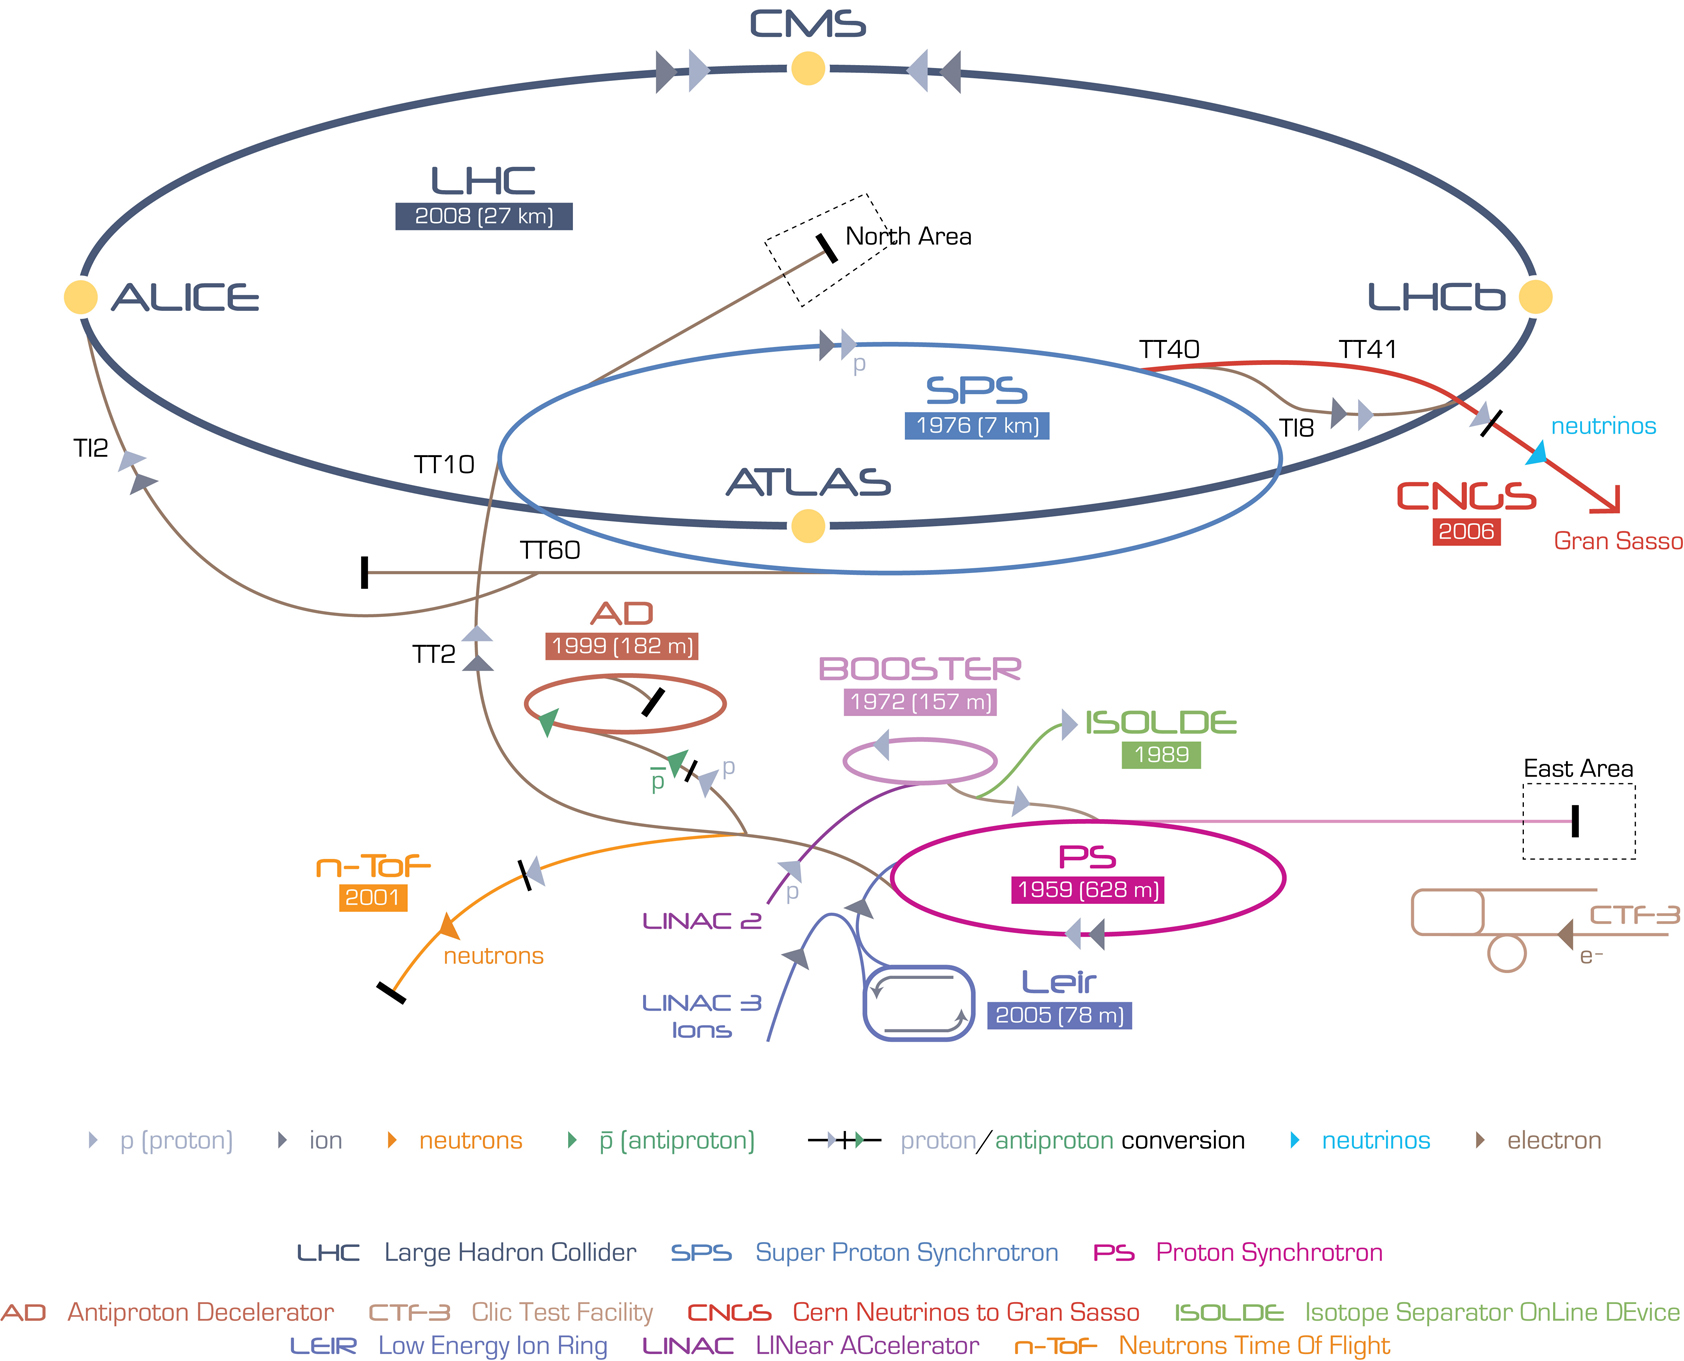
\includegraphics[width=0.8\textwidth]{Figures/LHC.jpg}
		%\rule{35em}{0.5pt}
	\caption[Schematics of Large Hadron Collider]{Schematics of Large Hadron Collider}
	\label{fig:LHC}
\end{figure}
%----------------------------------------------------------------------------------------
%	SECTION 1
%----------------------------------------------------------------------------------------

\section{Design of the Large Hadron Collider}

The Standard model of elementary particles describes nicely all known particles and interactions, however there are still some unanswered questions. One of the major question was the existence of Higgs boson which was solved in the past few years with the discovery of a new particle at 125 GeV. Other questions that is still open is the unification of fundamental forces, as it is difficult to construct a theory of gravity which would be similar to those of other fundamental interactions. One attempt to achieve this goal is the theory of supersymmetry which predicts that each particle has its heavier supersymetric partner which according to some theories could unify all fundamental forces. If the theory of supersymetry is correct, lightest supersymetic particles could be found at the LHC.  



\begin{figure}[htbp]
	\centering
		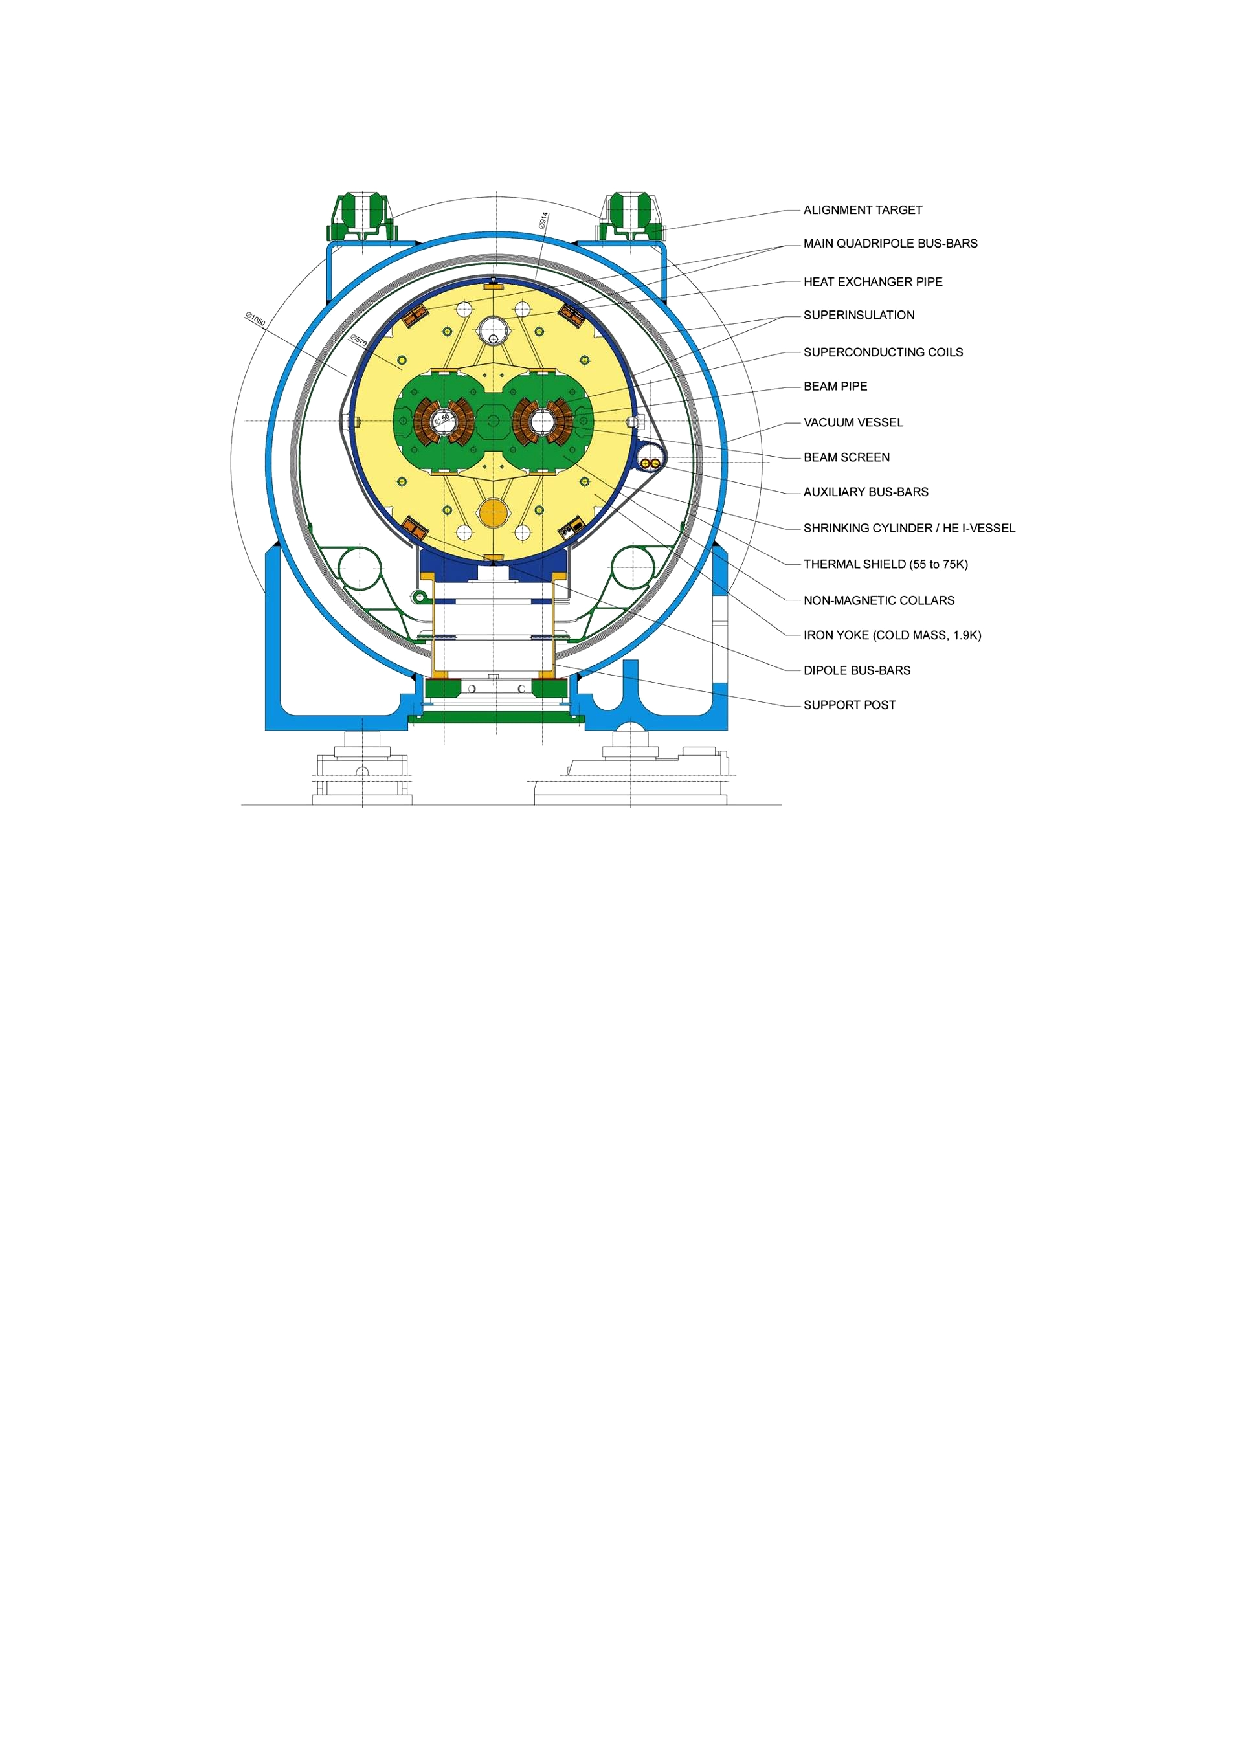
\includegraphics[width=0.7\textwidth]{Figures/LHC_magnet.pdf}
		%\rule{35em}{0.5pt}
	\caption[Schematics of dipole magnets]{Schematics of Dipole magnets}
	\label{fig:LHC_mag}
\end{figure}

%-----------------------------------
%	SECTION 2
%-----------------------------------

\section{Performance}

Since the start of the LHC in 2009, there were three years of machine operation, which yielded many physics results among which the discovery of Higgs boson reported by ATLAS and CMS collaborations. should be highlighted. First year of operation was devoted to commissioning and understanding machine characteristics with the emphasis on safety and testing machine protection systems. In 2011 new energy and instantaneous luminosity records were reached. These numbers were increased once again in 2012 with center of mass energy going to 8 TeV.
\par High bunch intensity with 50 ns bunch spacing was used in order to get a good instantaneous luminosity performance. This came at a cost of high number of collisions in one bunch crossing (pile-up) which was in 2012 around 12 collisions, and in some cases this number went as high as 20 interactions. With the increase of instantaneous luminosity in 2012, number of pile-up interactions was on the average around 30. Besides proton-proton collisions, LHC successfully delivered lead-lead ion runs in 2010 and 2011. primarily for the ALICE experiment, but also for CMS and ATLAS. At the start of 2013. there was also a successful proton-lead run performed for the first time. 

\begin{table}[h]
\centering
  \caption{LHC performance in 2012}
  \begin{tabular}{ l  c  c }
      \hline
      \hline
      Parameter & Design value & Value in 2012 \\
      \hline
      Beam energy [TeV] & 7 & 4 \\
      Bunch spacing [ns] & 25 & 50 \\
      Number of bunches & 2808 & 1374 \\
      Protons per bunch & 1.15$\times 10^{11}$ & 1.6-1.7$\times 10^{11}$ \\
      Peak luminosity [cm$^{-2}$s$^{-1}$] & 1$\times 10^{34}$ & 7.7$\times 10^{33}$ \\
      Max. number of events per bunch crossing & 19 & $\approx 40$ \\
      Stored beam energy [MJ] & 362 & $\approx$ 140 \\
      \hline
      \hline 
  \end{tabular}
\end{table}

LHC head achieved very good luminosity performance during pat years mainly because of the excellent beam quality delivered by the injectors with significantly more protons than nominal and with lower emittances. Since the LHC was capable to absorb these beams, it was chosen to continue to operate with 50 ns bunch spacing. This meant higher pile-up which had to be dealt with by the experiments. 


\begin{table}[h]
\centering
  \caption{LHC performance highlights}
  \begin{tabular}{ l  c }
      \hline
      \hline
      Max. luminosity delivered in one fill & 237 pb$^{-1}$  \\
      Max. luminosity delivered in 7 days & 1.35 fb$^{-1}$  \\
      Longest time in stable beams (2012) & 22.8 hours \\
      Longest time in stable beams over 7 days & 91.8 hours (55$\%$) \\
      \hline
      \hline 
  \end{tabular}
\end{table}

\begin{figure}[htbp]
	\centering
		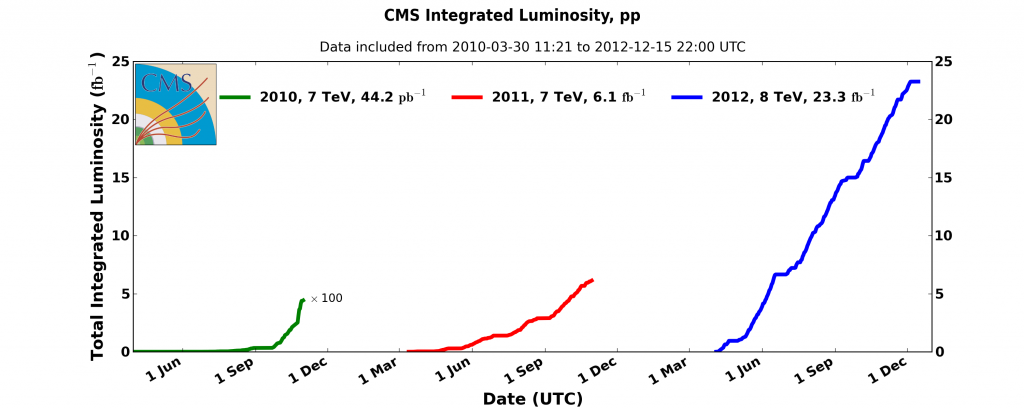
\includegraphics[width=0.7\textwidth]{Figures/lumi.png}
		%\rule{35em}{0.5pt}
	\caption[Luminosity delivered to the CMS experiment]{Luminosity delivered to the CMS experiment}
	\label{fig:LHC_lumi}
\end{figure}
 
Following a two year shutdown, LHC is anticipating operations at even higher energies of 6.5 TeV and later 7 TeV. The long term plan includes even higher peak luminosities, installation of the new injector complex and later the beginning of HL-LHC era. The timeline will, of course, be highly affected by the performance and results of the next run.